\chapter{Introducción}
\label{cap:capitulo1}
\setcounter{page}{1}

\begin{flushright}
\begin{minipage}[]{10cm}
\emph{Quizás algún fragmento de libro inspirador...}\\
\end{minipage}\\

Autor, \textit{Título}\\
\end{flushright}

\vspace{1cm}

La robótica se define como la intersección entre ciencia, ingeniería y tecnología con el objetivo de desarrollar máquinas que realicen tareas de forma automática. El término robot proviene de la palabra checa \textit{robota} que significa \textit{trabajo forzado}, se utilizó por primera vez en la obra de teatro RUR (Rossum's Universal Robots) del autor Karel Capek estrenada en 1921.\\

Se puede clasificar a los robots en dos grandes campos: robots industriales y robots de servicio. Según la norma internacional ISO 8373:2012 un robot industrial es un manipulador multifuncional, reprogramable y controlado automáticamente, programable en tres o más ejes que puede estar fijo en un área o móvil para su uso en aplicaciones de automatización industrial. Por otro lado, según la Federación Internacional de Robótica (IFR), un robot de servicio es un robot que opera de forma parcial o totalmente autónoma para realizar servicios útiles para el bienestar de los humanos y del equipamiento, excluyendo operaciones de manufactura.\\

En este primer capítulo se pretende dar un contexto amplio al lector sobre el presente trabajo. El autor comenzará presentando la robótica de servicio, campo para el cual está enfocado nuestro sistema, y continuará avanzando por los distintos conceptos generales hasta los más específicos.

\section{Robótica de servicio}
\label{sec:robotica} % etiqueta para luego referenciar esta sección

En los últimos años la robótica de servicio está obteniendo un auge exponencial, cada vez son más los campos en los que los robots ayudan a los seres humanos intentando mejorar su calidad de vida ayudándoles a realizar tareas peligrosas o proporcionando una compañía agradable a aquellos que lo necesitan. Entre las aplicaciones más importantes encontramos:

\begin{itemize}
 \item \textit{Limpieza.} Aspiradoras domésticas como iRobot Roomba 980 o limpiadores de ventanas como WinBot 950 (Figura \ref{fig:robots_limpieza}). Robots caracterizados por típicamente realizar tareas de navegación con el objetivo de recorrer completamente una zona mientras llevan a cabo las labores de limpieza.\\
 
\begin{figure} [h!]
  \begin{center}
    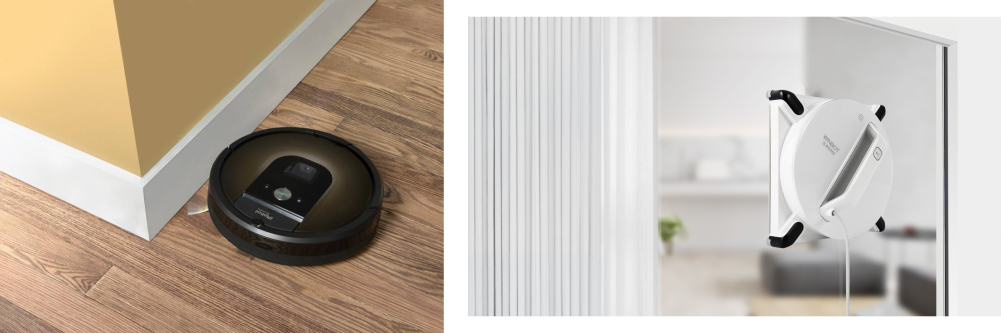
\includegraphics[width=12cm]{figs/robots_limpieza.png}
  \end{center}
  \caption{iRobot Roomba 980 y WinBot 950.}
  \label{fig:robots_limpieza}
\end{figure}

\item \textit{Inspección.} Cartografías 3D, inspección de plantas petrolíferas, aerogeneradores o minas. Suelen ser lugares de difícil acceso para los humanos, por lo tanto son tareas que estarán al cargo de robots cuadrúpedos o drones. Los robots con cuatro patas son actualmente los autómatas terrestres más estables del mercado y tienen la capacidad de recorrer terrenos inestables o incluso subir y bajar escales.  Uno de los más populares es Spot de Boston Dynamics (Figura \ref{fig:spot}).\\

\begin{figure} [h!]
  \begin{center}
    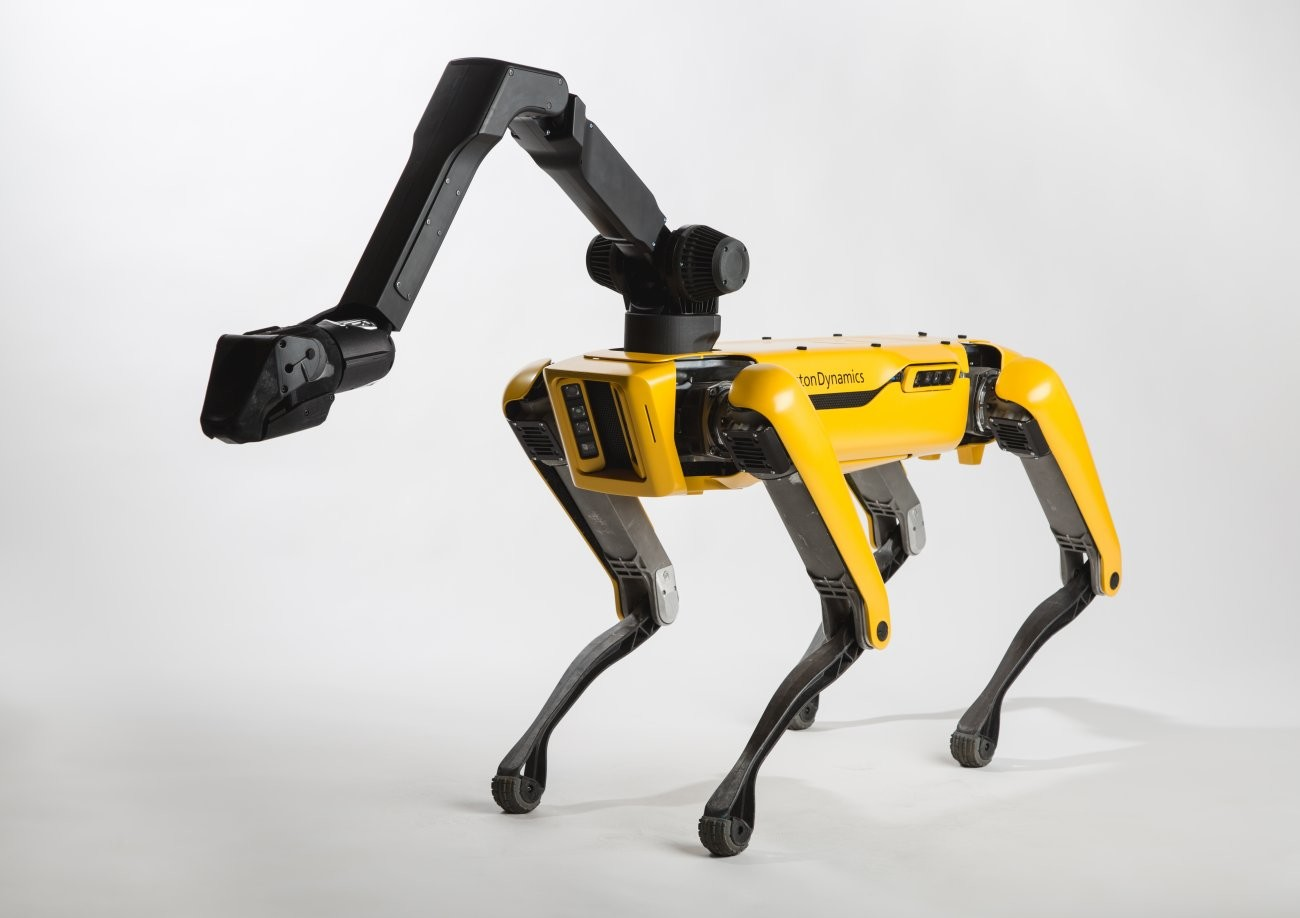
\includegraphics[width=8cm]{figs/spot.jpg}
  \end{center}
  \caption{Robot Spot de Boston Dynamics. Fuente \cite{xataka}}
  \label{fig:spot}
\end{figure}

\item \textit{Eduación.} Aquellos enfocados a la docencia tanto infantil como universitaria. Podemos destacar modelos como mBot con posibilidad de programación a través de bloques con mBlock IDE\footnote{\url{https://ide.mblock.cc}} o modelos como el TurtleBot con soporte ROS\footnote{\url{https://www.ros.org/}}.

\item \textit{Conducción autónoma.} Una tecnología cada vez más madura y extendida. Empresas como Waymo (Figura \ref{fig:waymo}) o AutoX ya están comercializando productos reales que llevan a cabo esta tarea proporcionando servicios de taxi autónomos. Otros fabricantes como Tesla comercializan también coches semi-automáticos.\\

\begin{figure} [h!]
  \begin{center}
    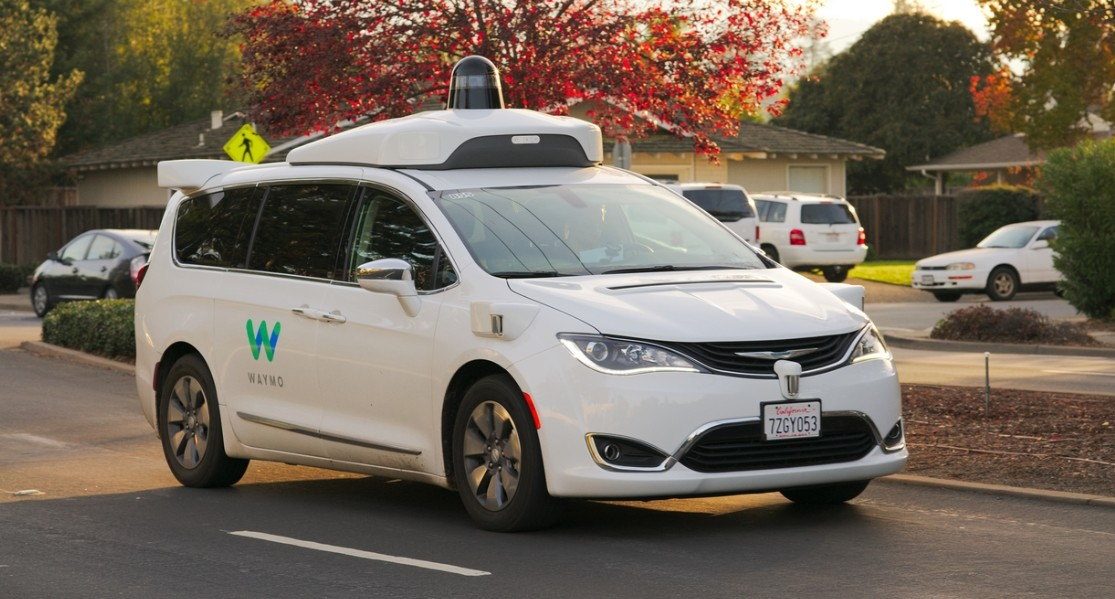
\includegraphics[width=8cm]{figs/waymo.jpg}
  \end{center}
  \caption{Taxi autónomo de Waymo. Fuente \cite{xataka}}
  \label{fig:waymo}
\end{figure}

\item \textit{Logística.} Robots destinados a agilizar el transporte de materiales o productos dentro de una fábrica o almacén. Existen dos grandes grupos: AGV (Vehículo Guiado Automático) y AMR (Robot Móvil Autónomo).

\item \textit{Ámbito sanitario.} Es uno de los campos más amplios dentro de la robótica de servicio, existen autómatas realizando múltiples tareas. Podemos encontrar exoesqueletos enfocados en la rehabilitación de la marcha humana como el Atlas de Marsi-Bionics o robots ayudantes en cirugía como Da Vinci o Mako (Figura \ref{fig:robots_cirugia}).

\begin{figure} [h!]
  \begin{center}
    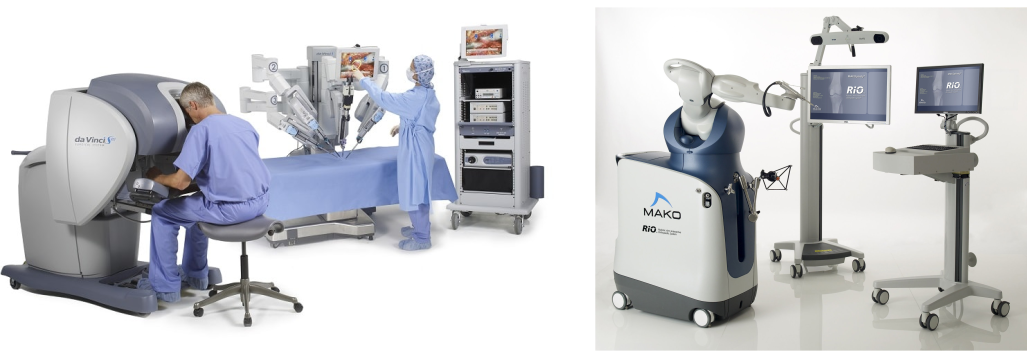
\includegraphics[width=12cm]{figs/robots_cirugia.png}
  \end{center}
  \caption{Robot DaVinci y Robot Mako. Fuente \cite{davinci} \cite{mako}}
  \label{fig:robots_cirugia}
\end{figure}

Además, en los últimos años está surgiendo y avanzando un nuevo tipo de robótica sanitaria, los robots de compañía o asistentes personales. Estos consiguen empatizar con los pacientes y hacerles pasar un rato más ameno o ayudarles a que no se sientan sólos. Para ello es indispensable realizar un buen HRI (Human Robot Interaction, en inglés), tema del cual trata la siguiente sección. Un ejemplo de robot de compañía sería Robin (Figura \ref{fig:robin}), el cual ayuda a los niños a superar el miedo de ir al médico.

\begin{figure} [h!]
  \begin{center}
    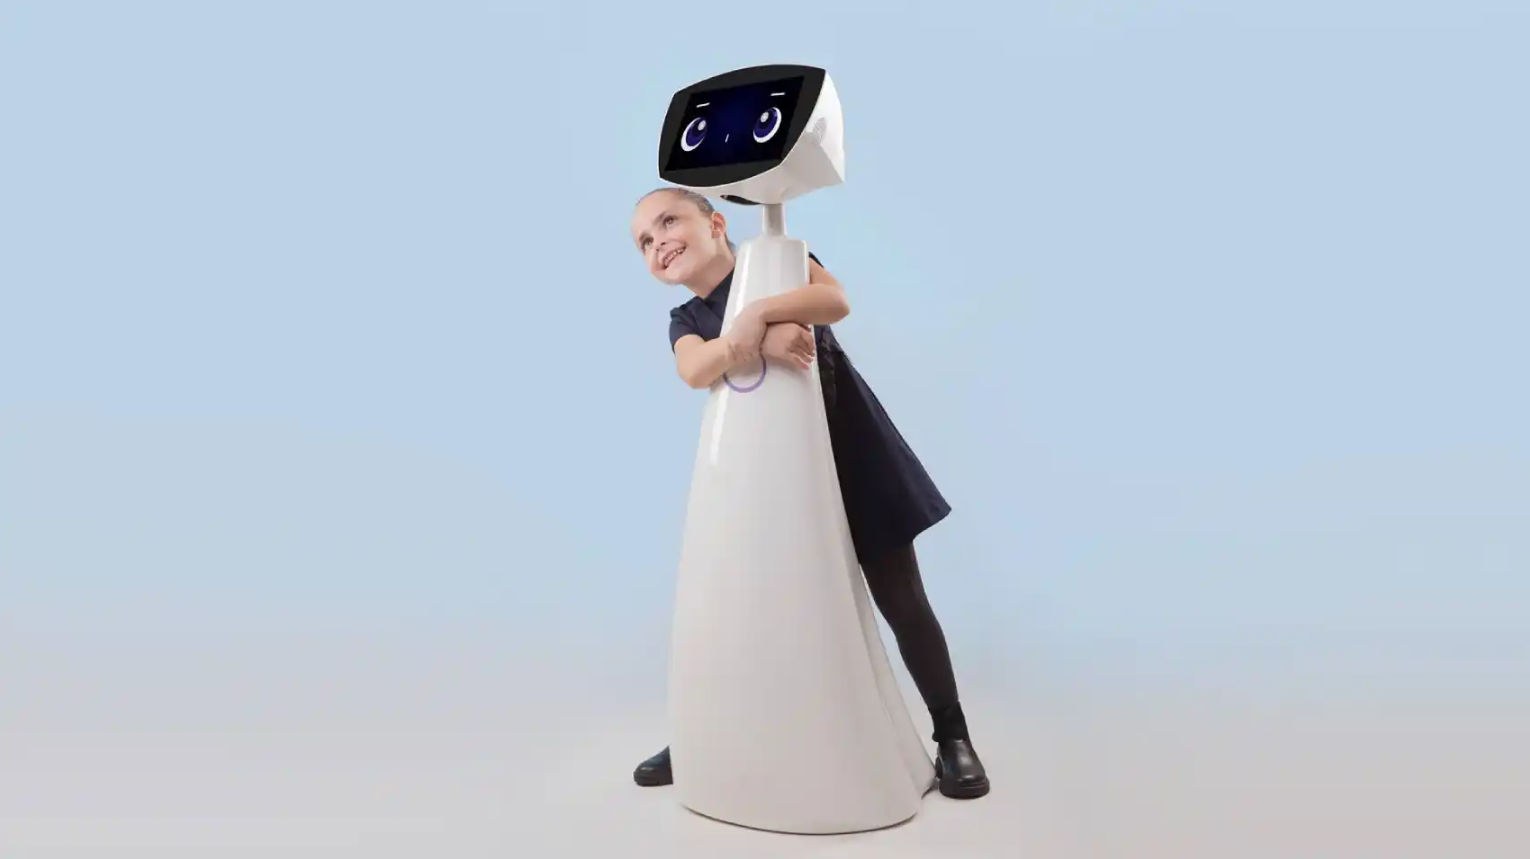
\includegraphics[width=9cm]{figs/robin.png}
  \end{center}
  \caption{Robot Robin.}
  \label{fig:robin}
\end{figure}
\end{itemize}

\section{Interacción Humano Robot (HRI)}
\label{sec:interaccion_humano_robot}

Podemos definir el HRI como el campo de estudio que intenta comprender, diseñar y evaluar la interacción entre los robots y los seres humanos. Debido a que los robots están cada vez más presentes en nuestras vidas, esta rama de investigación nace con la necesidad de que estos tengan la capacidad de colaborar y vivir con nosotros, los humanos.\\

La definición de HRI se remonta al año 1941, donde Isaac Asimov habla por primera vez de ello en su novela \textit{Yo, Robot}. Además escribe unas leyes, las que se conocen actualmente como \textit{Las Tres Leyes de la Robótica}, que promueven una interacción segura entre humanos y robots. Las tres leyes son las siguientes:

\begin{itemize}
    \item \textit{Primera Ley.} Un robot no hará daño a un ser humano ni, por inacción, permitirá que un ser humano sufra daño.
    \item \textit{Segunda Ley.} Un robot debe cumplir las órdenes dadas por los seres humanos, a excepción de aquellas que entren en conflicto con la primera ley.
    \item \textit{Tercera Ley.} Un robot debe proteger su propia existencia en la medida en que esta protección no entre en conflicto con la primera o la segunda ley.
\end{itemize}

Actualmente esas leyes representan el código moral y han sido modificadas por Isaac Asimov y otros autores para conseguir mayor perfección. Además Asimov agregó una cuarta ley por encima de esas tres que viene a ser una generalización de la primera, \textit{La Ley Cero}:

\begin{itemize}
    \item \textit{Ley Cero.} Un robot no puede dañar a la humanidad o, por inacción, permitir que la humanidad sufra daños.
\end{itemize}

En el artículo \cite{hri_distancing} se realiza un estudio enfocado en como el trato proporcionado por un robot a un humano influía en la distancia física de ambos. Para realizar los experimentos usaron un robot que era capaz de expresar emociones a través de gestos y los resultados demostraron que si el robot ejercía un trato poco social y nada empático, la distancia con el humano aumentaba. En cambio, si el robot expresaba un comportamiento amigable y comprensivo, la distancia con el humano disminuía ya que el nivel de confianza con el robot aumentaba. Por lo tanto si lo que queremos es que los robots sean capaces de colaborar y vivir con nosotros, debemos ser capaces de que estos actúen con empatía, comprensión y amabilidad hacia los seres humanos. Esto no es una tarea trivial, es más bien complicada, y surgen muchos baches por el camino.

\subsection{Problemática. Paradoja de Moravec}

Según Dautenhahn el robot debe adaptarse a nuestra forma de expresión y nos debe comprender tal como somos y actuamos. Esto es algo realmente complicado para una máquina ya que no tienen la capacidad de razonar, únicamente se limitan a ejecutar órdenes que previamente han sido programadas, y las reglas de un entorno social humano pueden ser muy variadas y poco esperadas. Este problema lo presenta la \textit{Paradoja de Moravec}.\\

Según Moravec los actos voluntarios de un humano requieren de poca computación para una máquina, mientras que los actos no conscientes e involuntarios requieren de grandes esfuerzos computacionales. Moravec afirmó <<comparativamente es fácil conseguir que las computadoras muestren capacidades similares a las de un humano adulto en tests de inteligencia, y difícil o imposible lograr que posean las habilidades perceptivas y motrices de un bebé de un año>> \cite{moravec}. Esto según él, es debido a la evolución biológica humana.\\

Todas nuestras habilidades han sido perfeccionadas a lo largo de millones de años por el proceso de selección natural y por lo tanto, sería lógico pensar que si intentamos replicar dichas habilidades en una máquina nos tomaría como mínimo el mismo tiempo proporcionalmente. Muchas de nuestras acciones más valiosas (coger objetos, reconocer voces, prestar atención, habilidades sociales...) son involuntarias y es eso lo que provoca que aplicarles ingeniería inversa sea muy complicado. Sin embargo habilidades como las matemáticas resultan complejas para nosotros, ya que nuestro cuerpo y cerebro no está preparado para ello, y muy triviales para las máquinas.\\

Conociendo toda esta problemática parece casi imposible que un robot sea capaz de interaccionar con un humano, pero existen últimos avances en la ingeniería que aportan un poco de claridad y optimismo al HRI.

\subsection{Soluciones robóticas de interacción}

Una interacción completa de humano-humano está regida por la vista, el oído y el tacto. Esos tres sentidos proporcionan toda la información que posteriormente nuestro cerebro procesará y razonará. Podemos concluir diciendo entonces que la interacción entre un humano y un robot estará compuesta por dos fases: \textit{percepción} y \textit{razonamiento}. Además después de haber razonado habría que actuar adecuadamente para que la interacción prosiga, pero no es un tema relevante en el contexto de este trabajo. 

\subsubsection{Percepción} 

Lo que para nosotros serían los sentidos, en los robots lo podemos sustituir por sensores. Cámaras para la vista, micrófonos para el oído o sensores de presión para el tacto. Además de estos existen múltiples variantes más y con mayor o menor precisión en su tarea. Podríamos decir que esta fase de la interacción está bastante bien cubierta y de algún modo es muy semejante a la humana.\\

Estos sensores por si sólos no tienen ningún valor sino que detrás de todos esos datos capturados deben existir algoritmos que saquen conclusiones de todos ellos. Por ejemplo, en los fotogramas capturados por una cámara se puede realizar detección de objetos o personas a través de la Visión Artificial y el Machine Learning. O por ejemplo, extraer palabras o frases del audio capturado por un micrófono usando también Machine Learning.\\

Podríamos pensar que esto ya nos resuelve todos los problemas, pero no es así. Hasta ahora sólo tenemos muchos datos sin ningún contexto, cosa que los humanos hacemos a través de la razón.

\subsubsection{Razonamiento} 

Sin lugar a dudas es la más compleja y la que más investigación necesita. A día de hoy no se ha conseguido implementar un real razonamiento humano dentro de un robot, pero si que se utilizan diversos trucos que simulan ese \textit{razonamiento}:

\begin{itemize}
\item \textit{Contexto de una conversación.} La frase <<No he visto ninguno>> puede tener múltiples significados dependiendo del tema el cual se esté tratando en la conversación. Se podría estar expresando que no se ha visto ningún error en la carta que se escribiendo o que no se ha visto llegar el taxi se había pedido. Entonces los robots no se pueden dedicar a detectar únicamente frases sueltas y actuar ante ellas. Para ello existen modelos de lenguaje como GPT-3 entrenados a través de Machine Learning que consiguen simular que están entendiendo el diálogo, pero en realidad sólo están repitiendo conversaciones con las que han sido entrenados.

\item \textit{Atención.} Mediante reconocimiento facial (usando Visión Artificial y Machine Learning) el robot puede realizar un seguimiento con la mirada a la cara del sujeto con el que está interactuando. Esto por ejemplo, simularía que el robot está prestando atención a una conversación.

\item \textit{Compresión de la situación emocional.} A través de la detección de emociones o expresiones faciales (otra vez usando Visión Artificial y Machine Learning) del sujeto con el que se está interactuando, el robot puede actuar de una manera u otra simulando que está comprendiendo situación emocional. El sistema de detección de emociones desarrollado en este trabajo estaría presente en este apartado y el anterior de \textit{Atención}.
\end{itemize}

Se ha comprobado que la Visión Artificial y el Machine Learning son temas clave en el desarrollo del sistema del presente trabajo. Ambos son introducidos en las próximas dos secciones.

\section{Visión Artificial}

Los seres humanos utilizamos nuestros ojos para, de alguna manera, comprender todo aquello que nos rodea. El objetivo de la visión artificial es trasladar esa misma habilidad a una máquina, osea, que sea capaz de percibir información visual del entorno y actuar según la situación. Para ello se realiza lo que se conoce como procesamiento de imagen, este se puede dividir en las siguientes fases o etapas:

\begin{itemize}
    \item \textit{Digitalización.} Proceso de transformación que sufre una imagen analógica a otra digital para que pueda ser manipulada por un ordenador. Una máquina sólo sabe comprender números, por lo tanto la imagen estará representada como una matriz de números (píxeles).
    
    \item \textit{Preprocesamiento.} En la etapa anterior es muy probable que las imágenes sufran degradaciones como pérdida de definición o aparición de ruido. Esta etapa intenta subsanarlas con técnicas como la reducción de ruido o realce del contraste.
    
    \item \textit{Segmentación.} Extracción de información contenida en la imagen mediante la descomposición de la misma en regiones significativas. Por ejemplo determinar en una imagen que píxeles pertenecen a los objetos y cuáles al fondo.
    
    \item \textit{Representación.} Tras realizar la segmentación se poseen píxeles en bruto. Se deberá elegir si se desean representar esos datos como el contorno de una región o como los puntos de dicha región. En eso consiste esta etapa.
    
    \item \textit{Descripción.} Selección de características o descriptores de la representación elegida para permitir la posterior clasificación de los objetos. Por ejemplo la cantidad de huecos o el perímetro del contorno.
    
    \item \textit{Reconocimiento.} Clasificación de los objetos de la imagen usando las características o descriptores obtenidos en la etapa anterior. A cada objeto se le asigna una etiqueta como \textit{Persona} o \textit{Planta}.
    
    \item \textit{Interpretación.} Etapa final, la cual se encarga de dar significado a los objetos reconocidos. Por ejemplo localizar que objetos son dinámicos o estáticos, o detectar la posición en la que se encuentra un cuerpo.
\end{itemize}

Lo explicado y desarrollado anteriormente se puede enmarcar dentro de lo que se conoce como la \textit{Visión Artificial Clásica}, enfocada en la utilización de algoritmos específicos para procesar imágenes y reconocer en ellas características básicas.\\

El auge de la Inteligencia Artificial (IA) y sobre todo el Machine Learning, está expandiendo exponencialmente las capacidades de la Visión Artificial. Sobre todo las Redes Neuronales Profundas o Deep Learning están aportado mucho valor en este campo. Son técnicas muy potentes que permiten resultados mucho mejores que los ofrecidos por la visión clásica y además mucho más fáciles de implementar. En la siguiente sección se introducirá dicho campo, el Machine Learning.

\section{Machine Learning}

El Machine Learning o Aprendizaje Automático es una disciplina del campo de la Inteligencia Artificial que permite a un ordenador realizar tareas de manera automática sin previamente haber sido programados explícitamente para dichos casos. Según el tipo de aprendizaje que realicen los algoritmos podemos clasificar estos en tres grandes grupos:

\begin{itemize}
\item \textit{Aprendizaje supervisado}
\item \textit{Aprendizaje no supervisado} 
\item \textit{Aprendizaje por refuerzo} 
\end{itemize}

Cada uno de los tipos de aprendizaje tiene determinadas características y diferentes aplicaciones finales que estudiaremos en la siguientes secciones.

\subsection{Aprendizaje supervisado}

Usado para resolver problemas conocidos. Se le proporciona al algoritmo un conjunto de datos de entrada y sus salidas correspondientes, entonces el algoritmo se dedica a \textit{aprender} la relación entre las salidas y las entradas. Generará unos patrones a partir de los cuales realizará predicciones.\\

Utilizando un ejemplo más familiar, si queremos que nuestro algoritmo aprenda a detectar gatos lo que debemos hacer es proporcionarle imágenes de ejemplo con gatos debidamente etiquetados. Una vez que el algoritmo haya recibido toda esa información y la haya procesado adecuadamente, la próxima vez que vea datos similares sabrá clasificarlos como gatos.\\

\noindent Dentro del aprendizaje supervisado se diferencian dos grandes tipos:
\begin{itemize}
\item \textit{\textbf{Regresión.}} Tiene como objetivo predecir la salida mediante una función que proporciona valores continuos. Por ejemplo predecir el precio de una vivienda a partir de su tamaño en metros cuadrados usando regresión lineal (Figura \ref{fig:ejemplo_regresion}).

\begin{figure} [h!]
  \begin{center}
    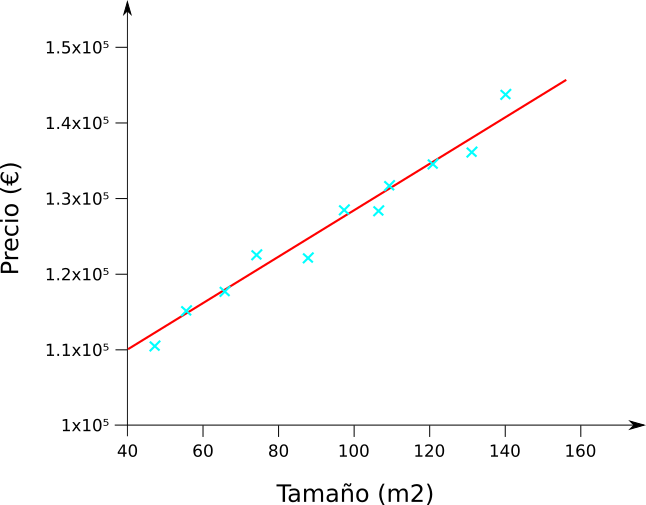
\includegraphics[width=9cm]{figs/ejemplo_regresion.png}
  \end{center}
  \caption{Ejemplo de regresión lineal.\\
  Predicción del precio de la vivienda.}
  \label{fig:ejemplo_regresion}
\end{figure}

En el ejemplo de la Figura \ref{fig:ejemplo_regresion} los datos usados como entrada serían los tamaños de las viviendas y los datos de salida los precios. Las cruces azules representan estos valores de entrada y salida y la línea roja representa la relación obtenida entre ellos. A partir de esa función lineal, el algoritmo ya sería capaz de realizar cualquier predicción para una pareja de datos de tamaño y precio.

Además de la regresión lineal, que es el ejemplo más simple, existen otros tipos como la regresión logística o la regresión polinomial.

\item \textit{\textbf{Clasificación.}} Las salidas toman valores discretos en función de los valores de entrada. Si la salida únicamente posee dos valores discretos, entonces estamos ante una clasificación binaria. Si la salida puede tomar más de dos valores discretos, la clasificación será multiclase.

Un ejemplo de clasificación binaria sería la predicción del tipo de casa (piso o chalet) en función de la distancia al centro de la ciudad y el tamaño del jardín (Figura \ref{fig:ejemplo_clasificacion_binaria}).

\begin{figure} [h!]
  \begin{center}
    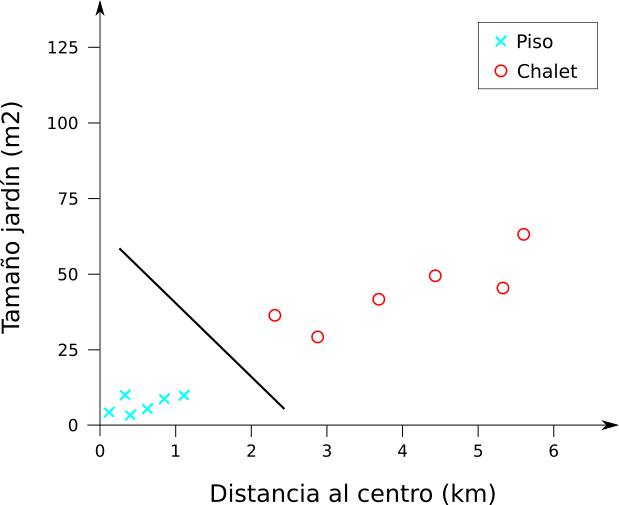
\includegraphics[width=9cm]{figs/ejemplo_clasificacion_binaria.png}
  \end{center}
  \caption{Ejemplo de clasificación binaria.\\
  Predicción del tipo de casa.}
  \label{fig:ejemplo_clasificacion_binaria}
\end{figure}

En el ejemplo de la Figura \ref{fig:ejemplo_clasificacion_binaria} los datos usados como entrada serían el tamaño del jardín y la distancia al centro y los datos de salida el tipo de casa. Se puede observar como el algoritmo de clasificación ha separado los datos en dos conjuntos diferenciados, cualquier dato nuevo que caiga en uno de esos conjuntos será clasificado con su etiqueta correspondiente. Es a eso a lo que se le llama predicción.

Los algoritmos más utilizados para realizar clasificación son SVM (Support Vector Machine), KNN (K Nearest Neighbour), Árboles de decisión y Redes Neuronales (Convolucionales, Recurrentes, etc.).

\end{itemize}

\subsection{Aprendizaje no supervisado}

Únicamente se le proporciona al algoritmo un conjunto de datos de entrada y el propio algoritmo será el encargado de detectar patrones dentro de ese conjunto. A diferencia del aprendizaje supervisado, aquí no existe ningún etiquetado de los datos, por lo tanto la máquina únicamente separara los datos por patrones pero no tendrá el concepto de que son gatos o perros.\\

Un ejemplo, siguiendo con la temática de las viviendas, sería agrupar las casas en función de la distancia al centro y del tamaño del jardín (Figura \ref{fig:ejemplo_clustering}). Esto se conoce como clustering o segmentación.\\

\begin{figure} [h!]
  \begin{center}
    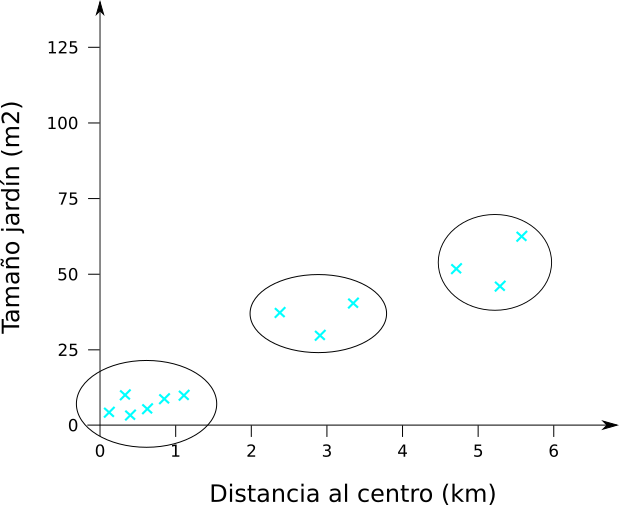
\includegraphics[width=9cm]{figs/ejemplo_no_supervisado.png}
  \end{center}
  \caption{Ejemplo de clustering.\\
            Agrupación de datos de casas.}
  \label{fig:ejemplo_clustering}
\end{figure}

En el ejemplo de la Figura \ref{fig:ejemplo_clustering} los datos de entrada serían el tamaño del jardín y la distancia al centro. Además al algoritmo, en este tipo de aprendizaje, se le suele indicar en cuántas clases se desea que se clasifiquen los datos. También se puede no indicar esta información y dejarle total libertad a la máquina. En este último caso los científicos de datos tiene la posibilidad de aprender más sobre estos y puede encontrar patrones interesantes u ocultos que antes no eran visibles.

\subsection{Aprendizaje por refuerzo}

No se le proporcionan datos de entrada ni de salida. El algoritmo aprende a desarrollar una tarea a partir de un esquema de recompensas y penalizaciones ante las decisiones que toma en cada una de las iteraciones. Ya no sólo se trata de clasificar unos datos en unas determinadas clases sino que tendremos muchos factores a la vez a los que prestar atención y actuar según la situación. Por eso este tipo de aprendizaje es sobre todo usado en robótica o videojuegos, ambos son máquinas o personajes actuando en un entorno cambiante.\\

A diferencia de los otros tipos de aprendizaje que se intenta reducir el error, aquí se intenta maximizar la recompensa. Los componentes del Aprendizaje Reforzado son:

\begin{itemize}
    \item \textit{\textbf{Agente.}} Modelo que se pretende entrenar para que aprendar a tomar decisiones.
    \item \textit{\textbf{Ambiente.}} Entorno donde interactúa el agente, el cual contiene las reglas posibles en cada momento.\\
\end{itemize}

Además la relación que se realimenta entre los componentes mencionados anteriormente cuenta con los siguientes nexos:

\begin{itemize}
    \item \textit{\textbf{Acción.}} Posibles acciones que puede tomar el Agente en un momento determinado.
    \item \textit{\textbf{Estado (del ambiente).}} Indicadores del ambiente de cómo están los elementos que lo componen en ese momento.
    \item \textit{\textbf{Recompensas o penalizaciones.}} Por cada acción tomada por el Agente, se obtendrá un premio o una penalización que orientará al Agente en si lo está haciendo bien o mal.
\end{itemize}

Se podría concluir afirmando que es una forma de entrenamiento basada en la fuerza bruta. Si el objetivo es que un robot recorra una habitación esquivando obstáculos, se le deberá someter a choques, acelerones, frenazos... para hacerle aprender lo que está bien y lo que está mal. El algoritmo más usado es Q-Learning.

\section{Sistemas embebidos}
Un sistema embebido (también conocido como \textit{empotrado}) es un sistema de computación diseñado para realizar funciones específicas, y cuyos componentes se encuentran integrados en una placa base. El procesamiento central del sistema se lleva a cabo gracias a un microcontrolador, es decir, un microprocesador que incluye además interfaces de entrada/salida, así como una memoria de tamaño reducido en el mismo chip \cite{sistemas_empotrados}.\\

Dependiendo del tipo de sistema embebido algunos pueden ser programados directamente en lenguaje ensamblador del microcontrolador o microprocesador u otros en lenguajes de más alto nivel como C++ o Python para desarrollo de aplicaciones.\\

Se comenzará definiendo lo que es un microprocesador y un microcontrolador. Es esencial entender ambos significados si se quiere saber en que consiste un sistema embebido.

\subsection{Microprocesador y microcontrolador}

Denominamos microprocesador al conjunto de elementos fusionados en un mismo circuito. Algunos de esos elementos la ALU (Unidad Aritmética Lógica) la cual se encarga de realizar las operaciones matemáticas o los registros que guardan los datos temporalmente. Normalmente conocemos a estos microprocesadores o procesadores como CPU (Unidad Central de Procesamiento) siendo el núcleo de nuestros ordenadores, esto es así ya que por sí sólos no tienen ningún uso, se integran junto a otros componentes que le dan el uso concreto final. Por ejemplo en un ordenador se integra junto con el disco duro, la memoria RAM, la tarjeta gráfica, y demás componentes.\\

Aquí es donde entra en juego el término de microcontrolador, podemos entenderlo como un pequeño ordenador con capacidad limitada. Si antes hablábamos del ordenador convencional esto lo podríamos entender igual pero todo integrado en un único chip. Es por ello que tendrán capacidad de cómputo limitada y no se les podrá someter a tareas muy exigentes. Sin embargo esto les proporciona una gran ventaja, su bajo coste económico. Por esto último es por lo que son tan populares y está en auge la investigación dedicada a intentar transportar tareas (que en principio necesitan de gran cómputo) a estos sistemas embebidos realizando las simplificaciones necesarias.

\subsection{Sistemas embebidos populares}
Existen múltiples fabricantes de sistemas empotrados, en este capítulo de introducción se nombraran los dos más grandes actualmente: Arduino\footnote{\url{https://www.arduino.cc/}} y Raspberry\footnote{\url{https://www.raspberrypi.org/}}. Ambos proporcionan microcontroladores aunque Raspberry es más conocida por sus SBC (Single Board Computer, en inglés).

\paragraph{Arduino.} Fabricante especializado en la venta de microcontroladores. Posee modelos como los Arduino UNO R3 (Figura \ref{fig:arduino_uno}) o Arduino Nano. Son microcontroladores integrados en el mismo chip con todos los componentes necesarios para su correcto funcionamiento (resistencias, condensadores, pines para conectar elementos, etc). Además de esto mencionado, la ventaja que nos proporciona este tipo de placas y Arduino es que a través de su entorno de desarrollo (Arduino IDE\footnote{\url{https://www.arduino.cc/en/software}}) tenemos la oportunidad de cargar código en los microcontroladores sin realizar métodos de ''flasheado'' y compilación tediosos que si requieren otro tipo de microcontroladores.

\begin{figure} [h!]
  \begin{center}
    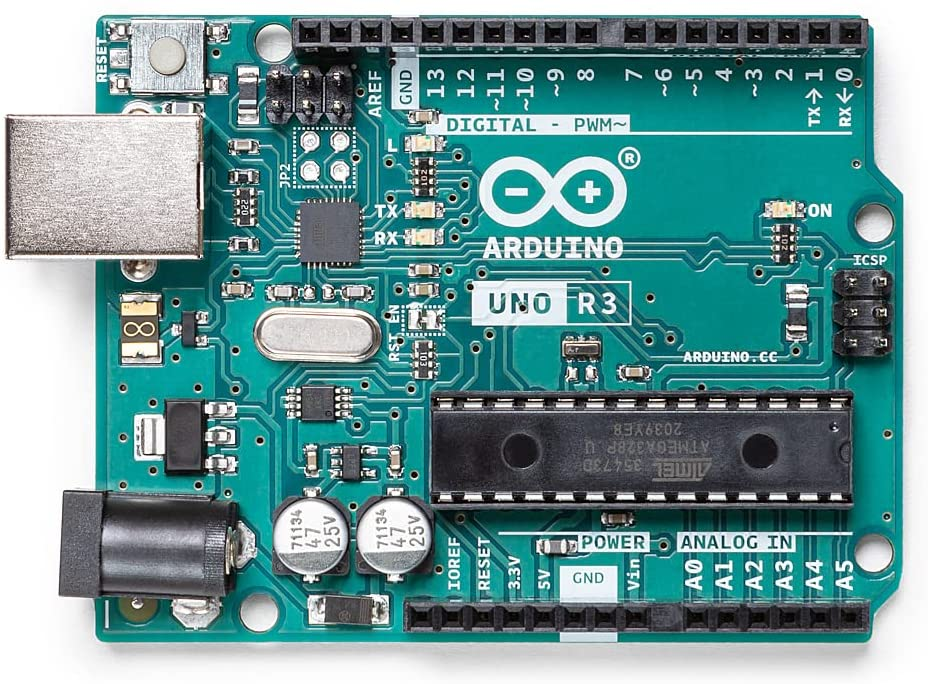
\includegraphics[width=9cm]{figs/arduino.jpg}
  \end{center}
  \caption{Microcontrolador Arduino UNO R3.}
  \label{fig:arduino_uno}
\end{figure}

\paragraph{Raspberry.} Tiene a la venta también microcontroladores como la Raspberry Pi Pico pero su producto principal son los SBC, su último modelo la Raspberry Pi 4b (Figura \ref{fig:raspberry}). El concepto es muy parecido al de Arduino pero con características más robustas, no sólo se trata de un microcontrolador simple, es un ordenador completo con su propio sistema operativo en una sola placa. Este mencionado sistema operativo es Raspberry Pi OS basado en Debian.

\begin{figure} [h!]
  \begin{center}
    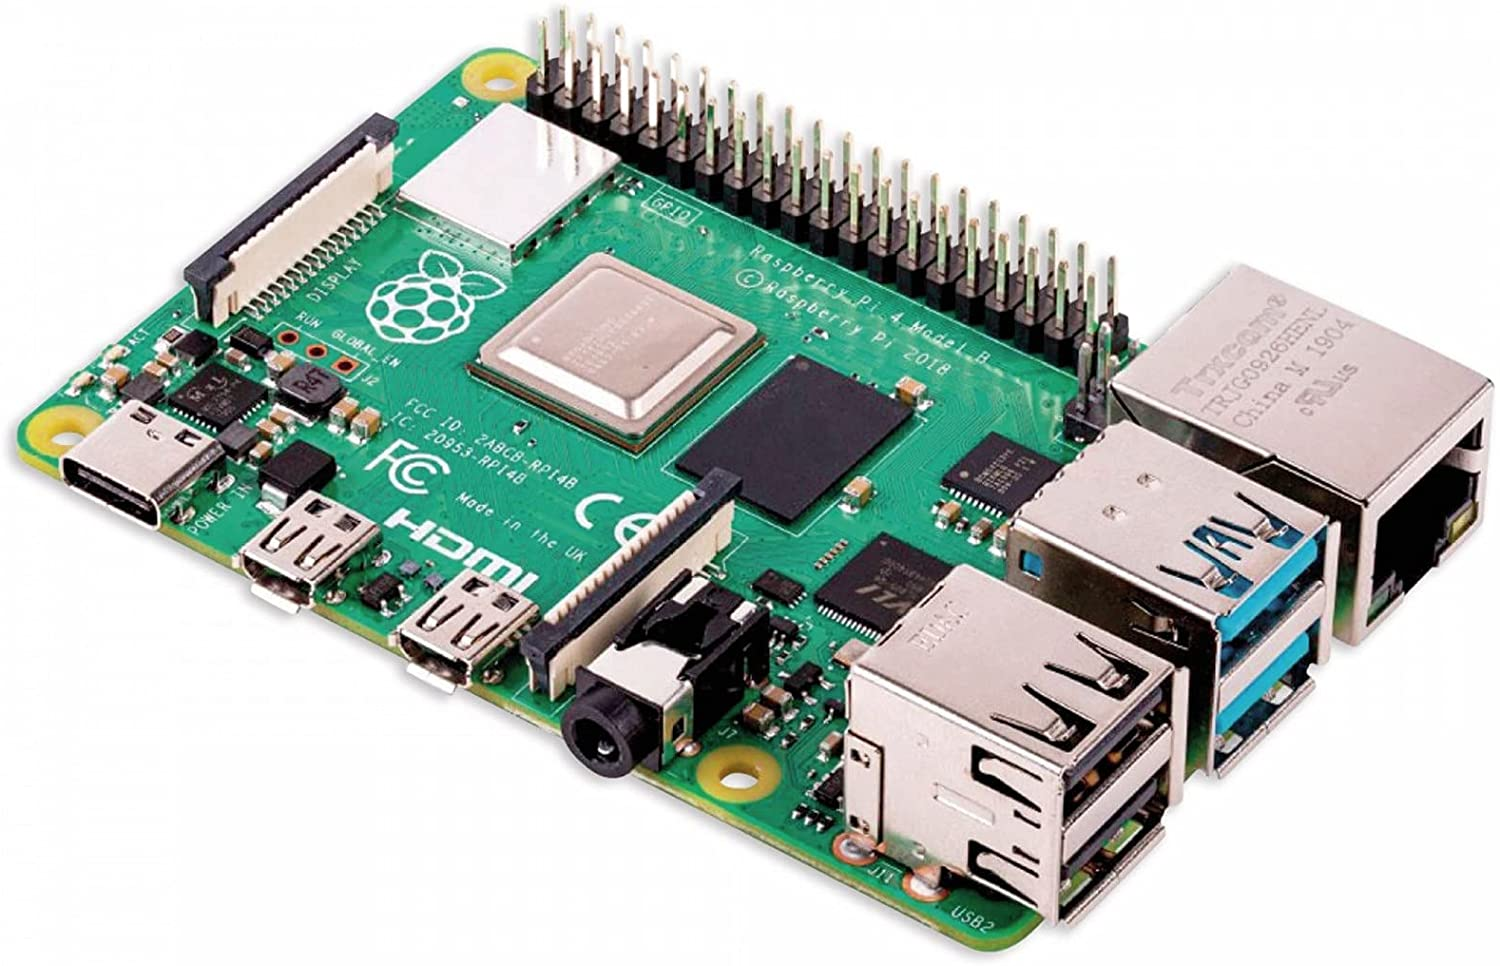
\includegraphics[width=9cm]{figs/raspberry.jpg}
  \end{center}
  \caption{Raspberry Pi 4b.}
  \label{fig:raspberry}
\end{figure}

En el siguiente capítulo (número 2) se realizará una descripción del problema a desarrollar y la metodología y el plan de trabajo que se ha llevado a cabo. Prosiguiendo con el capítulo 3, el autor expondrá las herramientas hardware y software utilizadas. En el capítulo 4 se mostrará todo el desarrollo del trabajo y los experimentos realizados. Por último, en el capítulo 5 se podrán encontrar las conclusiones finales.






